\section{Eksperymentalne wyznaczenie odpowiedzi skokowych}
\label{lab:zad2}

Przeprowadzono eksperyment mający na celu określenie wzmocnienia
sterowania. Ustawiono kolejno wartości sterowania równe: $20, 30 , 40, … , 80, 90$,
a następnie pozyskano wartości ustabilizowanego sygnału wyjściowego.


\subsection{Odpowiedzi skokowe}
\label{lab:zad2:odpSkok}

\begin{figure}[H] 
   \centering
   % This file was created by matlab2tikz.
%
\definecolor{mycolor1}{rgb}{0.00000,0.44700,0.74100}%
%
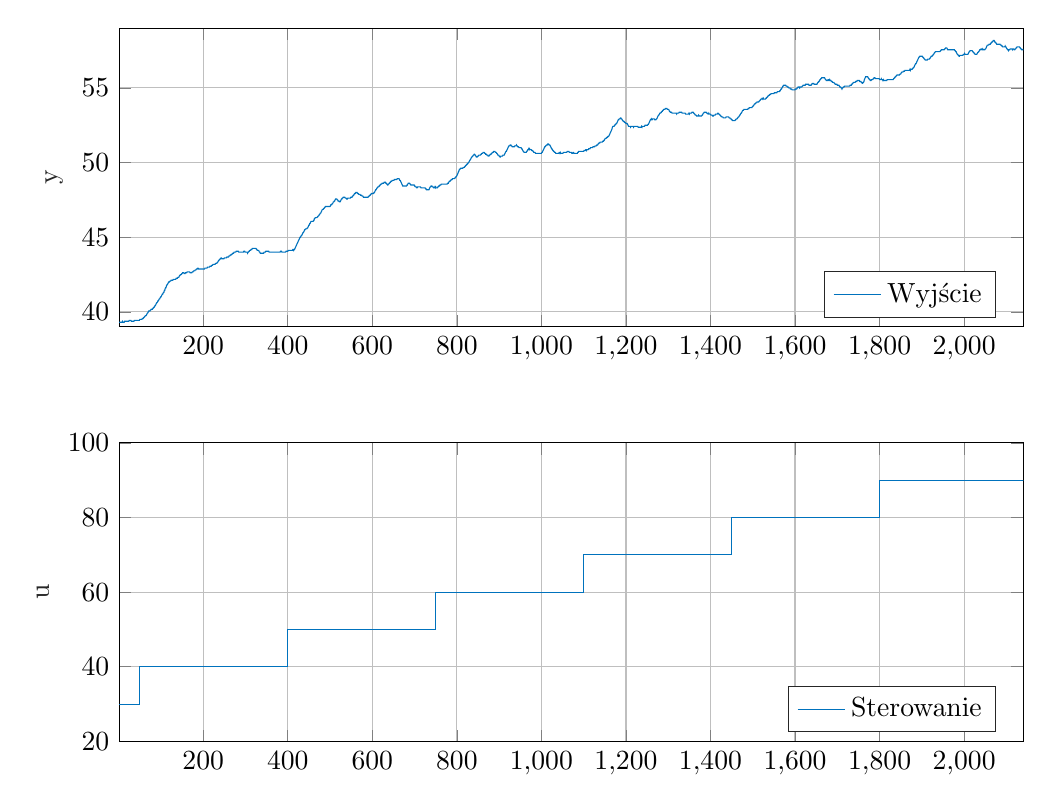
\begin{tikzpicture}

\begin{axis}[%
width=4.521in,
height=1.493in,
at={(0.758in,2.554in)},
scale only axis,
xmin=1,
xmax=2140,
ymin=39,
ymax=59,
ylabel style={font=\color{white!15!black}},
ylabel={y},
axis background/.style={fill=white},
xmajorgrids,
ymajorgrids,
legend style={at={(0.97,0.03)}, anchor=south east, legend cell align=left, align=left, draw=white!15!black}
]
\addplot [color=mycolor1]
  table[row sep=crcr]{%
1	39.31\\
2	39.31\\
3	39.31\\
4	39.31\\
5	39.31\\
6	39.31\\
7	39.31\\
8	39.31\\
9	39.37\\
10	39.31\\
11	39.31\\
12	39.31\\
13	39.31\\
14	39.37\\
15	39.37\\
16	39.37\\
17	39.37\\
18	39.37\\
19	39.37\\
20	39.37\\
21	39.37\\
22	39.37\\
23	39.37\\
24	39.37\\
25	39.43\\
26	39.43\\
27	39.43\\
28	39.43\\
29	39.43\\
30	39.37\\
31	39.37\\
32	39.37\\
33	39.37\\
34	39.37\\
35	39.37\\
36	39.37\\
37	39.43\\
38	39.43\\
39	39.43\\
40	39.43\\
41	39.43\\
42	39.43\\
43	39.43\\
44	39.43\\
45	39.43\\
46	39.43\\
47	39.43\\
48	39.43\\
49	39.43\\
50	39.5\\
51	39.5\\
52	39.5\\
53	39.5\\
54	39.5\\
55	39.5\\
56	39.56\\
57	39.56\\
58	39.56\\
59	39.62\\
60	39.62\\
61	39.68\\
62	39.68\\
63	39.75\\
64	39.75\\
65	39.75\\
66	39.81\\
67	39.87\\
68	39.93\\
69	39.93\\
70	40\\
71	40.06\\
72	40.06\\
73	40.06\\
74	40.06\\
75	40.12\\
76	40.12\\
77	40.18\\
78	40.18\\
79	40.18\\
80	40.18\\
81	40.25\\
82	40.25\\
83	40.31\\
84	40.31\\
85	40.37\\
86	40.43\\
87	40.43\\
88	40.5\\
89	40.56\\
90	40.62\\
91	40.62\\
92	40.68\\
93	40.75\\
94	40.75\\
95	40.81\\
96	40.87\\
97	40.87\\
98	40.93\\
99	41\\
100	41\\
101	41.06\\
102	41.12\\
103	41.18\\
104	41.18\\
105	41.25\\
106	41.31\\
107	41.31\\
108	41.43\\
109	41.43\\
110	41.56\\
111	41.62\\
112	41.62\\
113	41.75\\
114	41.81\\
115	41.81\\
116	41.87\\
117	41.93\\
118	42\\
119	42\\
120	42\\
121	42.06\\
122	42.06\\
123	42.06\\
124	42.12\\
125	42.12\\
126	42.12\\
127	42.12\\
128	42.12\\
129	42.18\\
130	42.18\\
131	42.18\\
132	42.18\\
133	42.18\\
134	42.18\\
135	42.18\\
136	42.25\\
137	42.25\\
138	42.25\\
139	42.25\\
140	42.31\\
141	42.31\\
142	42.31\\
143	42.37\\
144	42.43\\
145	42.43\\
146	42.5\\
147	42.5\\
148	42.5\\
149	42.56\\
150	42.56\\
151	42.62\\
152	42.62\\
153	42.62\\
154	42.62\\
155	42.56\\
156	42.56\\
157	42.56\\
158	42.62\\
159	42.62\\
160	42.62\\
161	42.62\\
162	42.68\\
163	42.68\\
164	42.68\\
165	42.68\\
166	42.68\\
167	42.68\\
168	42.68\\
169	42.62\\
170	42.62\\
171	42.62\\
172	42.62\\
173	42.62\\
174	42.68\\
175	42.68\\
176	42.68\\
177	42.75\\
178	42.75\\
179	42.75\\
180	42.75\\
181	42.81\\
182	42.81\\
183	42.81\\
184	42.87\\
185	42.87\\
186	42.87\\
187	42.93\\
188	42.93\\
189	42.87\\
190	42.87\\
191	42.87\\
192	42.87\\
193	42.87\\
194	42.87\\
195	42.87\\
196	42.87\\
197	42.87\\
198	42.87\\
199	42.87\\
200	42.87\\
201	42.87\\
202	42.87\\
203	42.87\\
204	42.93\\
205	42.93\\
206	42.93\\
207	42.93\\
208	42.93\\
209	42.93\\
210	43\\
211	43\\
212	43\\
213	43\\
214	43\\
215	43\\
216	43.06\\
217	43.06\\
218	43.06\\
219	43.06\\
220	43.12\\
221	43.12\\
222	43.12\\
223	43.18\\
224	43.18\\
225	43.18\\
226	43.18\\
227	43.18\\
228	43.18\\
229	43.25\\
230	43.25\\
231	43.25\\
232	43.25\\
233	43.31\\
234	43.31\\
235	43.37\\
236	43.43\\
237	43.43\\
238	43.5\\
239	43.5\\
240	43.56\\
241	43.56\\
242	43.62\\
243	43.62\\
244	43.56\\
245	43.56\\
246	43.56\\
247	43.56\\
248	43.56\\
249	43.56\\
250	43.62\\
251	43.62\\
252	43.62\\
253	43.62\\
254	43.62\\
255	43.62\\
256	43.68\\
257	43.68\\
258	43.68\\
259	43.68\\
260	43.68\\
261	43.75\\
262	43.75\\
263	43.75\\
264	43.81\\
265	43.81\\
266	43.81\\
267	43.87\\
268	43.87\\
269	43.87\\
270	43.93\\
271	43.93\\
272	43.93\\
273	44\\
274	44\\
275	44\\
276	44\\
277	44\\
278	44.06\\
279	44.06\\
280	44.06\\
281	44.06\\
282	44.06\\
283	44.06\\
284	44\\
285	44\\
286	44\\
287	44\\
288	44\\
289	44\\
290	44\\
291	44\\
292	44\\
293	44\\
294	44\\
295	44\\
296	44.06\\
297	44.06\\
298	44.06\\
299	44\\
300	44\\
301	44\\
302	44\\
303	44\\
304	44\\
305	43.93\\
306	44\\
307	44\\
308	44.06\\
309	44.06\\
310	44.12\\
311	44.12\\
312	44.12\\
313	44.18\\
314	44.18\\
315	44.18\\
316	44.25\\
317	44.25\\
318	44.25\\
319	44.25\\
320	44.25\\
321	44.25\\
322	44.25\\
323	44.25\\
324	44.25\\
325	44.25\\
326	44.18\\
327	44.18\\
328	44.12\\
329	44.12\\
330	44.12\\
331	44.12\\
332	44.06\\
333	44\\
334	44\\
335	43.93\\
336	43.93\\
337	43.93\\
338	43.93\\
339	43.93\\
340	43.93\\
341	43.93\\
342	43.93\\
343	43.93\\
344	44\\
345	44\\
346	44\\
347	44\\
348	44.06\\
349	44.06\\
350	44.06\\
351	44.06\\
352	44.06\\
353	44.06\\
354	44.06\\
355	44.06\\
356	44\\
357	44\\
358	44\\
359	44\\
360	44\\
361	44\\
362	44\\
363	44\\
364	44\\
365	44\\
366	44\\
367	44\\
368	44\\
369	44\\
370	44\\
371	44\\
372	44\\
373	44\\
374	44\\
375	44\\
376	44\\
377	44\\
378	44\\
379	44\\
380	44\\
381	44\\
382	44\\
383	44.06\\
384	44.06\\
385	44.06\\
386	44\\
387	44\\
388	44\\
389	44\\
390	44\\
391	44\\
392	44\\
393	44\\
394	44\\
395	44\\
396	44.06\\
397	44.06\\
398	44.06\\
399	44.06\\
400	44.06\\
401	44.12\\
402	44.12\\
403	44.12\\
404	44.12\\
405	44.12\\
406	44.12\\
407	44.12\\
408	44.12\\
409	44.12\\
410	44.12\\
411	44.12\\
412	44.18\\
413	44.18\\
414	44.12\\
415	44.18\\
416	44.18\\
417	44.25\\
418	44.31\\
419	44.37\\
420	44.43\\
421	44.5\\
422	44.56\\
423	44.62\\
424	44.68\\
425	44.75\\
426	44.81\\
427	44.87\\
428	44.93\\
429	45\\
430	45\\
431	45.06\\
432	45.12\\
433	45.12\\
434	45.18\\
435	45.25\\
436	45.31\\
437	45.31\\
438	45.37\\
439	45.43\\
440	45.5\\
441	45.5\\
442	45.56\\
443	45.56\\
444	45.56\\
445	45.56\\
446	45.62\\
447	45.62\\
448	45.68\\
449	45.75\\
450	45.81\\
451	45.81\\
452	45.93\\
453	45.93\\
454	46\\
455	46.06\\
456	46.06\\
457	46.06\\
458	46.06\\
459	46.06\\
460	46.06\\
461	46.12\\
462	46.12\\
463	46.25\\
464	46.25\\
465	46.31\\
466	46.31\\
467	46.31\\
468	46.31\\
469	46.31\\
470	46.37\\
471	46.37\\
472	46.43\\
473	46.43\\
474	46.5\\
475	46.5\\
476	46.56\\
477	46.62\\
478	46.62\\
479	46.68\\
480	46.75\\
481	46.81\\
482	46.87\\
483	46.87\\
484	46.87\\
485	46.93\\
486	46.93\\
487	47\\
488	47\\
489	47.06\\
490	47.06\\
491	47.06\\
492	47.06\\
493	47.06\\
494	47.06\\
495	47.06\\
496	47.06\\
497	47.06\\
498	47.06\\
499	47.06\\
500	47.06\\
501	47.12\\
502	47.18\\
503	47.18\\
504	47.18\\
505	47.25\\
506	47.25\\
507	47.31\\
508	47.37\\
509	47.37\\
510	47.43\\
511	47.43\\
512	47.5\\
513	47.56\\
514	47.56\\
515	47.56\\
516	47.56\\
517	47.5\\
518	47.5\\
519	47.43\\
520	47.43\\
521	47.43\\
522	47.37\\
523	47.37\\
524	47.37\\
525	47.43\\
526	47.5\\
527	47.56\\
528	47.56\\
529	47.62\\
530	47.62\\
531	47.68\\
532	47.68\\
533	47.68\\
534	47.68\\
535	47.68\\
536	47.62\\
537	47.62\\
538	47.62\\
539	47.56\\
540	47.56\\
541	47.56\\
542	47.62\\
543	47.62\\
544	47.62\\
545	47.62\\
546	47.62\\
547	47.62\\
548	47.62\\
549	47.68\\
550	47.68\\
551	47.68\\
552	47.68\\
553	47.75\\
554	47.75\\
555	47.81\\
556	47.81\\
557	47.87\\
558	47.93\\
559	47.93\\
560	47.93\\
561	48\\
562	48\\
563	48\\
564	48\\
565	47.93\\
566	47.93\\
567	47.93\\
568	47.87\\
569	47.87\\
570	47.87\\
571	47.87\\
572	47.81\\
573	47.81\\
574	47.81\\
575	47.81\\
576	47.75\\
577	47.75\\
578	47.75\\
579	47.68\\
580	47.68\\
581	47.68\\
582	47.68\\
583	47.68\\
584	47.68\\
585	47.68\\
586	47.68\\
587	47.68\\
588	47.68\\
589	47.68\\
590	47.68\\
591	47.75\\
592	47.75\\
593	47.75\\
594	47.81\\
595	47.81\\
596	47.87\\
597	47.87\\
598	47.93\\
599	47.93\\
600	47.93\\
601	47.93\\
602	47.93\\
603	47.93\\
604	48\\
605	48\\
606	48.06\\
607	48.12\\
608	48.18\\
609	48.18\\
610	48.25\\
611	48.31\\
612	48.31\\
613	48.37\\
614	48.37\\
615	48.37\\
616	48.43\\
617	48.43\\
618	48.5\\
619	48.5\\
620	48.56\\
621	48.56\\
622	48.56\\
623	48.62\\
624	48.62\\
625	48.62\\
626	48.62\\
627	48.62\\
628	48.68\\
629	48.68\\
630	48.68\\
631	48.68\\
632	48.62\\
633	48.62\\
634	48.56\\
635	48.56\\
636	48.5\\
637	48.5\\
638	48.56\\
639	48.56\\
640	48.62\\
641	48.62\\
642	48.68\\
643	48.68\\
644	48.75\\
645	48.75\\
646	48.75\\
647	48.81\\
648	48.81\\
649	48.81\\
650	48.81\\
651	48.81\\
652	48.87\\
653	48.87\\
654	48.87\\
655	48.87\\
656	48.87\\
657	48.87\\
658	48.87\\
659	48.93\\
660	48.93\\
661	48.93\\
662	48.93\\
663	48.93\\
664	48.87\\
665	48.81\\
666	48.81\\
667	48.75\\
668	48.68\\
669	48.62\\
670	48.56\\
671	48.5\\
672	48.43\\
673	48.43\\
674	48.43\\
675	48.43\\
676	48.43\\
677	48.43\\
678	48.43\\
679	48.43\\
680	48.43\\
681	48.43\\
682	48.5\\
683	48.5\\
684	48.56\\
685	48.62\\
686	48.62\\
687	48.62\\
688	48.62\\
689	48.56\\
690	48.56\\
691	48.5\\
692	48.5\\
693	48.5\\
694	48.5\\
695	48.5\\
696	48.5\\
697	48.5\\
698	48.5\\
699	48.5\\
700	48.43\\
701	48.43\\
702	48.37\\
703	48.37\\
704	48.37\\
705	48.31\\
706	48.31\\
707	48.37\\
708	48.37\\
709	48.37\\
710	48.37\\
711	48.37\\
712	48.37\\
713	48.37\\
714	48.37\\
715	48.31\\
716	48.31\\
717	48.31\\
718	48.31\\
719	48.31\\
720	48.31\\
721	48.31\\
722	48.31\\
723	48.31\\
724	48.31\\
725	48.31\\
726	48.25\\
727	48.25\\
728	48.18\\
729	48.18\\
730	48.18\\
731	48.18\\
732	48.18\\
733	48.18\\
734	48.18\\
735	48.25\\
736	48.31\\
737	48.37\\
738	48.37\\
739	48.43\\
740	48.43\\
741	48.43\\
742	48.37\\
743	48.37\\
744	48.37\\
745	48.31\\
746	48.31\\
747	48.31\\
748	48.37\\
749	48.31\\
750	48.37\\
751	48.31\\
752	48.31\\
753	48.31\\
754	48.31\\
755	48.37\\
756	48.37\\
757	48.43\\
758	48.43\\
759	48.43\\
760	48.5\\
761	48.5\\
762	48.5\\
763	48.56\\
764	48.56\\
765	48.56\\
766	48.56\\
767	48.56\\
768	48.56\\
769	48.56\\
770	48.56\\
771	48.56\\
772	48.56\\
773	48.56\\
774	48.56\\
775	48.56\\
776	48.56\\
777	48.56\\
778	48.62\\
779	48.62\\
780	48.62\\
781	48.68\\
782	48.75\\
783	48.75\\
784	48.75\\
785	48.81\\
786	48.81\\
787	48.87\\
788	48.87\\
789	48.87\\
790	48.93\\
791	48.93\\
792	48.93\\
793	48.93\\
794	48.93\\
795	48.93\\
796	49\\
797	49\\
798	49.06\\
799	49.06\\
800	49.12\\
801	49.18\\
802	49.25\\
803	49.31\\
804	49.43\\
805	49.43\\
806	49.56\\
807	49.56\\
808	49.56\\
809	49.62\\
810	49.62\\
811	49.62\\
812	49.62\\
813	49.62\\
814	49.62\\
815	49.68\\
816	49.68\\
817	49.68\\
818	49.68\\
819	49.75\\
820	49.75\\
821	49.81\\
822	49.81\\
823	49.87\\
824	49.87\\
825	49.93\\
826	49.93\\
827	50\\
828	50\\
829	50.06\\
830	50.12\\
831	50.18\\
832	50.18\\
833	50.25\\
834	50.31\\
835	50.37\\
836	50.37\\
837	50.43\\
838	50.43\\
839	50.5\\
840	50.5\\
841	50.56\\
842	50.56\\
843	50.5\\
844	50.5\\
845	50.43\\
846	50.37\\
847	50.37\\
848	50.37\\
849	50.43\\
850	50.43\\
851	50.43\\
852	50.5\\
853	50.5\\
854	50.5\\
855	50.5\\
856	50.5\\
857	50.56\\
858	50.56\\
859	50.62\\
860	50.62\\
861	50.62\\
862	50.68\\
863	50.68\\
864	50.68\\
865	50.68\\
866	50.62\\
867	50.62\\
868	50.56\\
869	50.56\\
870	50.56\\
871	50.5\\
872	50.5\\
873	50.5\\
874	50.43\\
875	50.43\\
876	50.43\\
877	50.5\\
878	50.5\\
879	50.56\\
880	50.56\\
881	50.56\\
882	50.62\\
883	50.62\\
884	50.68\\
885	50.68\\
886	50.68\\
887	50.75\\
888	50.75\\
889	50.75\\
890	50.75\\
891	50.68\\
892	50.68\\
893	50.68\\
894	50.62\\
895	50.62\\
896	50.56\\
897	50.5\\
898	50.5\\
899	50.5\\
900	50.43\\
901	50.43\\
902	50.37\\
903	50.37\\
904	50.43\\
905	50.43\\
906	50.43\\
907	50.43\\
908	50.43\\
909	50.5\\
910	50.5\\
911	50.5\\
912	50.5\\
913	50.56\\
914	50.62\\
915	50.68\\
916	50.75\\
917	50.75\\
918	50.81\\
919	50.87\\
920	50.93\\
921	51\\
922	51.06\\
923	51.12\\
924	51.12\\
925	51.12\\
926	51.18\\
927	51.18\\
928	51.18\\
929	51.12\\
930	51.12\\
931	51.06\\
932	51.06\\
933	51.06\\
934	51.06\\
935	51.06\\
936	51.06\\
937	51.12\\
938	51.12\\
939	51.12\\
940	51.12\\
941	51.18\\
942	51.12\\
943	51.12\\
944	51.06\\
945	51.06\\
946	51.06\\
947	51\\
948	51\\
949	51\\
950	51\\
951	51\\
952	51\\
953	50.93\\
954	50.93\\
955	50.87\\
956	50.81\\
957	50.75\\
958	50.75\\
959	50.68\\
960	50.68\\
961	50.68\\
962	50.68\\
963	50.68\\
964	50.68\\
965	50.75\\
966	50.75\\
967	50.81\\
968	50.87\\
969	50.87\\
970	50.93\\
971	50.87\\
972	50.93\\
973	50.87\\
974	50.87\\
975	50.87\\
976	50.87\\
977	50.81\\
978	50.81\\
979	50.81\\
980	50.75\\
981	50.75\\
982	50.68\\
983	50.68\\
984	50.68\\
985	50.68\\
986	50.62\\
987	50.62\\
988	50.62\\
989	50.62\\
990	50.62\\
991	50.62\\
992	50.62\\
993	50.62\\
994	50.62\\
995	50.62\\
996	50.62\\
997	50.62\\
998	50.62\\
999	50.62\\
1000	50.62\\
1001	50.68\\
1002	50.68\\
1003	50.75\\
1004	50.81\\
1005	50.87\\
1006	50.93\\
1007	51\\
1008	51.06\\
1009	51.06\\
1010	51.12\\
1011	51.12\\
1012	51.18\\
1013	51.18\\
1014	51.18\\
1015	51.25\\
1016	51.25\\
1017	51.25\\
1018	51.18\\
1019	51.18\\
1020	51.18\\
1021	51.12\\
1022	51.06\\
1023	51\\
1024	50.93\\
1025	50.93\\
1026	50.87\\
1027	50.81\\
1028	50.81\\
1029	50.75\\
1030	50.75\\
1031	50.68\\
1032	50.68\\
1033	50.68\\
1034	50.62\\
1035	50.62\\
1036	50.62\\
1037	50.62\\
1038	50.62\\
1039	50.62\\
1040	50.62\\
1041	50.62\\
1042	50.68\\
1043	50.68\\
1044	50.62\\
1045	50.68\\
1046	50.62\\
1047	50.62\\
1048	50.62\\
1049	50.62\\
1050	50.62\\
1051	50.62\\
1052	50.68\\
1053	50.68\\
1054	50.68\\
1055	50.68\\
1056	50.68\\
1057	50.68\\
1058	50.68\\
1059	50.68\\
1060	50.68\\
1061	50.75\\
1062	50.75\\
1063	50.75\\
1064	50.75\\
1065	50.75\\
1066	50.68\\
1067	50.68\\
1068	50.68\\
1069	50.68\\
1070	50.68\\
1071	50.68\\
1072	50.62\\
1073	50.62\\
1074	50.62\\
1075	50.68\\
1076	50.68\\
1077	50.62\\
1078	50.62\\
1079	50.62\\
1080	50.62\\
1081	50.62\\
1082	50.62\\
1083	50.62\\
1084	50.62\\
1085	50.62\\
1086	50.68\\
1087	50.68\\
1088	50.75\\
1089	50.75\\
1090	50.75\\
1091	50.75\\
1092	50.75\\
1093	50.75\\
1094	50.75\\
1095	50.75\\
1096	50.75\\
1097	50.75\\
1098	50.75\\
1099	50.75\\
1100	50.75\\
1101	50.81\\
1102	50.81\\
1103	50.81\\
1104	50.81\\
1105	50.87\\
1106	50.87\\
1107	50.81\\
1108	50.87\\
1109	50.87\\
1110	50.87\\
1111	50.87\\
1112	50.93\\
1113	50.93\\
1114	50.93\\
1115	50.93\\
1116	51\\
1117	51\\
1118	51\\
1119	51\\
1120	51\\
1121	51\\
1122	51.06\\
1123	51.06\\
1124	51.06\\
1125	51.06\\
1126	51.06\\
1127	51.12\\
1128	51.12\\
1129	51.12\\
1130	51.12\\
1131	51.18\\
1132	51.18\\
1133	51.18\\
1134	51.25\\
1135	51.25\\
1136	51.31\\
1137	51.31\\
1138	51.31\\
1139	51.37\\
1140	51.37\\
1141	51.37\\
1142	51.37\\
1143	51.37\\
1144	51.37\\
1145	51.43\\
1146	51.43\\
1147	51.43\\
1148	51.5\\
1149	51.5\\
1150	51.56\\
1151	51.62\\
1152	51.62\\
1153	51.62\\
1154	51.68\\
1155	51.68\\
1156	51.68\\
1157	51.75\\
1158	51.75\\
1159	51.75\\
1160	51.81\\
1161	51.87\\
1162	51.93\\
1163	52\\
1164	52.06\\
1165	52.12\\
1166	52.18\\
1167	52.25\\
1168	52.37\\
1169	52.43\\
1170	52.43\\
1171	52.43\\
1172	52.43\\
1173	52.5\\
1174	52.5\\
1175	52.56\\
1176	52.56\\
1177	52.62\\
1178	52.62\\
1179	52.68\\
1180	52.75\\
1181	52.81\\
1182	52.87\\
1183	52.87\\
1184	52.93\\
1185	52.93\\
1186	52.93\\
1187	53\\
1188	53\\
1189	52.93\\
1190	52.93\\
1191	52.87\\
1192	52.81\\
1193	52.81\\
1194	52.75\\
1195	52.75\\
1196	52.75\\
1197	52.68\\
1198	52.68\\
1199	52.68\\
1200	52.62\\
1201	52.62\\
1202	52.62\\
1203	52.62\\
1204	52.56\\
1205	52.5\\
1206	52.43\\
1207	52.43\\
1208	52.43\\
1209	52.43\\
1210	52.43\\
1211	52.37\\
1212	52.43\\
1213	52.43\\
1214	52.43\\
1215	52.43\\
1216	52.43\\
1217	52.43\\
1218	52.37\\
1219	52.43\\
1220	52.43\\
1221	52.43\\
1222	52.43\\
1223	52.43\\
1224	52.43\\
1225	52.43\\
1226	52.43\\
1227	52.43\\
1228	52.43\\
1229	52.37\\
1230	52.37\\
1231	52.37\\
1232	52.37\\
1233	52.37\\
1234	52.37\\
1235	52.37\\
1236	52.37\\
1237	52.43\\
1238	52.37\\
1239	52.43\\
1240	52.43\\
1241	52.43\\
1242	52.43\\
1243	52.43\\
1244	52.43\\
1245	52.5\\
1246	52.5\\
1247	52.5\\
1248	52.5\\
1249	52.5\\
1250	52.5\\
1251	52.5\\
1252	52.56\\
1253	52.56\\
1254	52.62\\
1255	52.68\\
1256	52.75\\
1257	52.81\\
1258	52.87\\
1259	52.87\\
1260	52.93\\
1261	52.87\\
1262	52.87\\
1263	52.93\\
1264	52.93\\
1265	52.93\\
1266	52.93\\
1267	52.93\\
1268	52.87\\
1269	52.87\\
1270	52.87\\
1271	52.87\\
1272	52.93\\
1273	52.93\\
1274	53\\
1275	53.06\\
1276	53.12\\
1277	53.18\\
1278	53.18\\
1279	53.25\\
1280	53.31\\
1281	53.31\\
1282	53.31\\
1283	53.37\\
1284	53.37\\
1285	53.43\\
1286	53.43\\
1287	53.5\\
1288	53.5\\
1289	53.56\\
1290	53.56\\
1291	53.56\\
1292	53.56\\
1293	53.62\\
1294	53.62\\
1295	53.62\\
1296	53.62\\
1297	53.62\\
1298	53.56\\
1299	53.56\\
1300	53.56\\
1301	53.56\\
1302	53.5\\
1303	53.43\\
1304	53.43\\
1305	53.37\\
1306	53.37\\
1307	53.37\\
1308	53.37\\
1309	53.31\\
1310	53.31\\
1311	53.31\\
1312	53.31\\
1313	53.31\\
1314	53.31\\
1315	53.31\\
1316	53.31\\
1317	53.31\\
1318	53.31\\
1319	53.31\\
1320	53.25\\
1321	53.31\\
1322	53.31\\
1323	53.31\\
1324	53.31\\
1325	53.31\\
1326	53.37\\
1327	53.37\\
1328	53.37\\
1329	53.37\\
1330	53.37\\
1331	53.37\\
1332	53.37\\
1333	53.31\\
1334	53.31\\
1335	53.31\\
1336	53.31\\
1337	53.31\\
1338	53.31\\
1339	53.31\\
1340	53.31\\
1341	53.25\\
1342	53.25\\
1343	53.25\\
1344	53.25\\
1345	53.25\\
1346	53.25\\
1347	53.25\\
1348	53.25\\
1349	53.31\\
1350	53.25\\
1351	53.31\\
1352	53.31\\
1353	53.31\\
1354	53.31\\
1355	53.31\\
1356	53.37\\
1357	53.37\\
1358	53.37\\
1359	53.37\\
1360	53.31\\
1361	53.31\\
1362	53.25\\
1363	53.25\\
1364	53.18\\
1365	53.18\\
1366	53.18\\
1367	53.12\\
1368	53.12\\
1369	53.12\\
1370	53.12\\
1371	53.12\\
1372	53.18\\
1373	53.12\\
1374	53.12\\
1375	53.12\\
1376	53.12\\
1377	53.12\\
1378	53.12\\
1379	53.12\\
1380	53.18\\
1381	53.18\\
1382	53.25\\
1383	53.31\\
1384	53.31\\
1385	53.37\\
1386	53.37\\
1387	53.37\\
1388	53.37\\
1389	53.37\\
1390	53.37\\
1391	53.31\\
1392	53.31\\
1393	53.31\\
1394	53.25\\
1395	53.25\\
1396	53.31\\
1397	53.25\\
1398	53.25\\
1399	53.25\\
1400	53.25\\
1401	53.18\\
1402	53.18\\
1403	53.18\\
1404	53.18\\
1405	53.12\\
1406	53.12\\
1407	53.12\\
1408	53.18\\
1409	53.18\\
1410	53.18\\
1411	53.18\\
1412	53.25\\
1413	53.25\\
1414	53.25\\
1415	53.25\\
1416	53.25\\
1417	53.31\\
1418	53.31\\
1419	53.25\\
1420	53.25\\
1421	53.25\\
1422	53.18\\
1423	53.18\\
1424	53.12\\
1425	53.12\\
1426	53.06\\
1427	53.06\\
1428	53.06\\
1429	53.06\\
1430	53\\
1431	53\\
1432	53\\
1433	53\\
1434	53\\
1435	53\\
1436	53\\
1437	53.06\\
1438	53.06\\
1439	53.06\\
1440	53.06\\
1441	53.06\\
1442	53.06\\
1443	53.06\\
1444	53\\
1445	53\\
1446	53\\
1447	52.93\\
1448	52.93\\
1449	52.93\\
1450	52.87\\
1451	52.87\\
1452	52.81\\
1453	52.81\\
1454	52.81\\
1455	52.81\\
1456	52.81\\
1457	52.81\\
1458	52.81\\
1459	52.87\\
1460	52.87\\
1461	52.93\\
1462	52.93\\
1463	52.93\\
1464	53\\
1465	53\\
1466	53.06\\
1467	53.06\\
1468	53.12\\
1469	53.18\\
1470	53.18\\
1471	53.25\\
1472	53.31\\
1473	53.31\\
1474	53.37\\
1475	53.43\\
1476	53.5\\
1477	53.5\\
1478	53.5\\
1479	53.56\\
1480	53.56\\
1481	53.56\\
1482	53.56\\
1483	53.56\\
1484	53.56\\
1485	53.56\\
1486	53.56\\
1487	53.56\\
1488	53.56\\
1489	53.62\\
1490	53.62\\
1491	53.62\\
1492	53.68\\
1493	53.68\\
1494	53.68\\
1495	53.68\\
1496	53.68\\
1497	53.68\\
1498	53.68\\
1499	53.75\\
1500	53.75\\
1501	53.81\\
1502	53.81\\
1503	53.87\\
1504	53.93\\
1505	53.93\\
1506	53.93\\
1507	54\\
1508	54\\
1509	54\\
1510	54.06\\
1511	54.06\\
1512	54.06\\
1513	54.06\\
1514	54.06\\
1515	54.12\\
1516	54.12\\
1517	54.18\\
1518	54.18\\
1519	54.25\\
1520	54.25\\
1521	54.25\\
1522	54.31\\
1523	54.31\\
1524	54.25\\
1525	54.31\\
1526	54.25\\
1527	54.25\\
1528	54.25\\
1529	54.25\\
1530	54.25\\
1531	54.31\\
1532	54.31\\
1533	54.37\\
1534	54.37\\
1535	54.43\\
1536	54.43\\
1537	54.5\\
1538	54.5\\
1539	54.5\\
1540	54.56\\
1541	54.56\\
1542	54.56\\
1543	54.62\\
1544	54.62\\
1545	54.62\\
1546	54.62\\
1547	54.62\\
1548	54.62\\
1549	54.62\\
1550	54.62\\
1551	54.68\\
1552	54.68\\
1553	54.68\\
1554	54.68\\
1555	54.68\\
1556	54.68\\
1557	54.68\\
1558	54.75\\
1559	54.75\\
1560	54.75\\
1561	54.75\\
1562	54.75\\
1563	54.75\\
1564	54.81\\
1565	54.81\\
1566	54.87\\
1567	54.93\\
1568	54.93\\
1569	55\\
1570	55.06\\
1571	55.12\\
1572	55.12\\
1573	55.18\\
1574	55.18\\
1575	55.18\\
1576	55.18\\
1577	55.18\\
1578	55.18\\
1579	55.12\\
1580	55.12\\
1581	55.12\\
1582	55.06\\
1583	55.06\\
1584	55.06\\
1585	55\\
1586	55\\
1587	55\\
1588	55\\
1589	54.93\\
1590	54.93\\
1591	54.93\\
1592	54.93\\
1593	54.87\\
1594	54.87\\
1595	54.87\\
1596	54.87\\
1597	54.87\\
1598	54.87\\
1599	54.87\\
1600	54.87\\
1601	54.93\\
1602	54.93\\
1603	54.93\\
1604	54.93\\
1605	55\\
1606	55\\
1607	55.06\\
1608	55.06\\
1609	55.06\\
1610	55.06\\
1611	55\\
1612	55.06\\
1613	55.06\\
1614	55.06\\
1615	55.06\\
1616	55.06\\
1617	55.12\\
1618	55.12\\
1619	55.18\\
1620	55.18\\
1621	55.18\\
1622	55.18\\
1623	55.18\\
1624	55.18\\
1625	55.25\\
1626	55.25\\
1627	55.25\\
1628	55.25\\
1629	55.25\\
1630	55.25\\
1631	55.25\\
1632	55.25\\
1633	55.18\\
1634	55.18\\
1635	55.18\\
1636	55.18\\
1637	55.18\\
1638	55.18\\
1639	55.25\\
1640	55.25\\
1641	55.31\\
1642	55.31\\
1643	55.31\\
1644	55.31\\
1645	55.25\\
1646	55.25\\
1647	55.25\\
1648	55.25\\
1649	55.25\\
1650	55.25\\
1651	55.25\\
1652	55.25\\
1653	55.31\\
1654	55.37\\
1655	55.37\\
1656	55.43\\
1657	55.43\\
1658	55.5\\
1659	55.56\\
1660	55.56\\
1661	55.62\\
1662	55.62\\
1663	55.68\\
1664	55.68\\
1665	55.68\\
1666	55.68\\
1667	55.68\\
1668	55.68\\
1669	55.68\\
1670	55.68\\
1671	55.62\\
1672	55.56\\
1673	55.56\\
1674	55.5\\
1675	55.5\\
1676	55.5\\
1677	55.5\\
1678	55.56\\
1679	55.56\\
1680	55.5\\
1681	55.5\\
1682	55.56\\
1683	55.5\\
1684	55.5\\
1685	55.5\\
1686	55.43\\
1687	55.43\\
1688	55.43\\
1689	55.37\\
1690	55.37\\
1691	55.37\\
1692	55.37\\
1693	55.31\\
1694	55.31\\
1695	55.25\\
1696	55.25\\
1697	55.25\\
1698	55.25\\
1699	55.25\\
1700	55.18\\
1701	55.18\\
1702	55.18\\
1703	55.18\\
1704	55.18\\
1705	55.12\\
1706	55.06\\
1707	55.06\\
1708	55.06\\
1709	55\\
1710	55\\
1711	54.93\\
1712	55\\
1713	55\\
1714	55.06\\
1715	55.06\\
1716	55.06\\
1717	55.12\\
1718	55.12\\
1719	55.12\\
1720	55.12\\
1721	55.12\\
1722	55.12\\
1723	55.12\\
1724	55.12\\
1725	55.12\\
1726	55.12\\
1727	55.12\\
1728	55.12\\
1729	55.12\\
1730	55.18\\
1731	55.18\\
1732	55.18\\
1733	55.18\\
1734	55.25\\
1735	55.25\\
1736	55.31\\
1737	55.31\\
1738	55.37\\
1739	55.37\\
1740	55.37\\
1741	55.37\\
1742	55.37\\
1743	55.43\\
1744	55.43\\
1745	55.43\\
1746	55.43\\
1747	55.5\\
1748	55.5\\
1749	55.5\\
1750	55.5\\
1751	55.5\\
1752	55.5\\
1753	55.43\\
1754	55.43\\
1755	55.43\\
1756	55.43\\
1757	55.37\\
1758	55.37\\
1759	55.31\\
1760	55.31\\
1761	55.37\\
1762	55.37\\
1763	55.43\\
1764	55.56\\
1765	55.62\\
1766	55.68\\
1767	55.75\\
1768	55.75\\
1769	55.75\\
1770	55.75\\
1771	55.75\\
1772	55.75\\
1773	55.68\\
1774	55.62\\
1775	55.62\\
1776	55.56\\
1777	55.56\\
1778	55.5\\
1779	55.5\\
1780	55.5\\
1781	55.56\\
1782	55.56\\
1783	55.56\\
1784	55.56\\
1785	55.62\\
1786	55.62\\
1787	55.68\\
1788	55.68\\
1789	55.68\\
1790	55.62\\
1791	55.62\\
1792	55.62\\
1793	55.62\\
1794	55.62\\
1795	55.62\\
1796	55.62\\
1797	55.62\\
1798	55.62\\
1799	55.62\\
1800	55.56\\
1801	55.56\\
1802	55.56\\
1803	55.56\\
1804	55.62\\
1805	55.56\\
1806	55.56\\
1807	55.56\\
1808	55.5\\
1809	55.56\\
1810	55.5\\
1811	55.5\\
1812	55.5\\
1813	55.5\\
1814	55.5\\
1815	55.5\\
1816	55.5\\
1817	55.5\\
1818	55.56\\
1819	55.56\\
1820	55.56\\
1821	55.56\\
1822	55.56\\
1823	55.56\\
1824	55.56\\
1825	55.56\\
1826	55.56\\
1827	55.56\\
1828	55.56\\
1829	55.56\\
1830	55.56\\
1831	55.56\\
1832	55.56\\
1833	55.62\\
1834	55.62\\
1835	55.68\\
1836	55.68\\
1837	55.75\\
1838	55.75\\
1839	55.81\\
1840	55.81\\
1841	55.87\\
1842	55.87\\
1843	55.87\\
1844	55.87\\
1845	55.87\\
1846	55.87\\
1847	55.87\\
1848	55.93\\
1849	55.93\\
1850	55.93\\
1851	56\\
1852	56.06\\
1853	56.06\\
1854	56.06\\
1855	56.06\\
1856	56.12\\
1857	56.12\\
1858	56.12\\
1859	56.12\\
1860	56.18\\
1861	56.18\\
1862	56.18\\
1863	56.18\\
1864	56.18\\
1865	56.18\\
1866	56.18\\
1867	56.18\\
1868	56.18\\
1869	56.18\\
1870	56.18\\
1871	56.18\\
1872	56.25\\
1873	56.18\\
1874	56.25\\
1875	56.25\\
1876	56.25\\
1877	56.25\\
1878	56.31\\
1879	56.31\\
1880	56.37\\
1881	56.37\\
1882	56.43\\
1883	56.5\\
1884	56.56\\
1885	56.62\\
1886	56.62\\
1887	56.68\\
1888	56.75\\
1889	56.81\\
1890	56.87\\
1891	56.93\\
1892	57\\
1893	57.06\\
1894	57.06\\
1895	57.12\\
1896	57.12\\
1897	57.12\\
1898	57.12\\
1899	57.12\\
1900	57.12\\
1901	57.12\\
1902	57.06\\
1903	57.06\\
1904	57\\
1905	57\\
1906	56.93\\
1907	56.93\\
1908	56.87\\
1909	56.87\\
1910	56.87\\
1911	56.87\\
1912	56.87\\
1913	56.87\\
1914	56.93\\
1915	56.93\\
1916	56.93\\
1917	56.93\\
1918	56.93\\
1919	57\\
1920	57\\
1921	57.06\\
1922	57.12\\
1923	57.12\\
1924	57.12\\
1925	57.18\\
1926	57.18\\
1927	57.25\\
1928	57.25\\
1929	57.31\\
1930	57.37\\
1931	57.37\\
1932	57.43\\
1933	57.43\\
1934	57.43\\
1935	57.43\\
1936	57.43\\
1937	57.43\\
1938	57.43\\
1939	57.43\\
1940	57.43\\
1941	57.43\\
1942	57.43\\
1943	57.43\\
1944	57.5\\
1945	57.5\\
1946	57.56\\
1947	57.56\\
1948	57.56\\
1949	57.56\\
1950	57.56\\
1951	57.56\\
1952	57.56\\
1953	57.56\\
1954	57.62\\
1955	57.62\\
1956	57.68\\
1957	57.68\\
1958	57.68\\
1959	57.68\\
1960	57.62\\
1961	57.56\\
1962	57.56\\
1963	57.56\\
1964	57.56\\
1965	57.56\\
1966	57.56\\
1967	57.56\\
1968	57.56\\
1969	57.56\\
1970	57.56\\
1971	57.56\\
1972	57.56\\
1973	57.56\\
1974	57.56\\
1975	57.56\\
1976	57.56\\
1977	57.56\\
1978	57.5\\
1979	57.5\\
1980	57.43\\
1981	57.43\\
1982	57.37\\
1983	57.31\\
1984	57.25\\
1985	57.25\\
1986	57.18\\
1987	57.18\\
1988	57.12\\
1989	57.12\\
1990	57.18\\
1991	57.18\\
1992	57.18\\
1993	57.18\\
1994	57.18\\
1995	57.18\\
1996	57.18\\
1997	57.18\\
1998	57.25\\
1999	57.25\\
2000	57.25\\
2001	57.31\\
2002	57.25\\
2003	57.25\\
2004	57.25\\
2005	57.25\\
2006	57.25\\
2007	57.25\\
2008	57.25\\
2009	57.25\\
2010	57.31\\
2011	57.37\\
2012	57.43\\
2013	57.43\\
2014	57.5\\
2015	57.5\\
2016	57.5\\
2017	57.5\\
2018	57.5\\
2019	57.5\\
2020	57.43\\
2021	57.43\\
2022	57.37\\
2023	57.37\\
2024	57.31\\
2025	57.31\\
2026	57.25\\
2027	57.25\\
2028	57.25\\
2029	57.25\\
2030	57.25\\
2031	57.31\\
2032	57.37\\
2033	57.37\\
2034	57.43\\
2035	57.43\\
2036	57.5\\
2037	57.56\\
2038	57.56\\
2039	57.56\\
2040	57.62\\
2041	57.62\\
2042	57.56\\
2043	57.56\\
2044	57.62\\
2045	57.56\\
2046	57.56\\
2047	57.56\\
2048	57.56\\
2049	57.56\\
2050	57.62\\
2051	57.62\\
2052	57.68\\
2053	57.75\\
2054	57.81\\
2055	57.87\\
2056	57.87\\
2057	57.87\\
2058	57.87\\
2059	57.93\\
2060	57.93\\
2061	57.93\\
2062	57.93\\
2063	58\\
2064	58\\
2065	58.06\\
2066	58.06\\
2067	58.12\\
2068	58.12\\
2069	58.18\\
2070	58.18\\
2071	58.18\\
2072	58.12\\
2073	58.06\\
2074	58.06\\
2075	58\\
2076	58\\
2077	57.93\\
2078	57.93\\
2079	57.93\\
2080	57.93\\
2081	57.93\\
2082	57.93\\
2083	57.93\\
2084	57.93\\
2085	57.93\\
2086	57.87\\
2087	57.87\\
2088	57.87\\
2089	57.81\\
2090	57.81\\
2091	57.75\\
2092	57.75\\
2093	57.75\\
2094	57.75\\
2095	57.75\\
2096	57.75\\
2097	57.81\\
2098	57.75\\
2099	57.75\\
2100	57.68\\
2101	57.62\\
2102	57.62\\
2103	57.56\\
2104	57.56\\
2105	57.5\\
2106	57.56\\
2107	57.56\\
2108	57.56\\
2109	57.62\\
2110	57.62\\
2111	57.62\\
2112	57.62\\
2113	57.62\\
2114	57.56\\
2115	57.62\\
2116	57.62\\
2117	57.62\\
2118	57.56\\
2119	57.56\\
2120	57.56\\
2121	57.62\\
2122	57.62\\
2123	57.68\\
2124	57.68\\
2125	57.75\\
2126	57.75\\
2127	57.75\\
2128	57.75\\
2129	57.75\\
2130	57.75\\
2131	57.75\\
2132	57.68\\
2133	57.68\\
2134	57.62\\
2135	57.62\\
2136	57.56\\
2137	57.56\\
2138	57.56\\
2139	57.56\\
2140	57.62\\
};
\addlegendentry{Wyjście}

\end{axis}

\begin{axis}[%
width=4.521in,
height=1.493in,
at={(0.758in,0.481in)},
scale only axis,
xmin=1,
xmax=2140,
ymin=20,
ymax=100,
ylabel style={font=\color{white!15!black}},
ylabel={u},
axis background/.style={fill=white},
xmajorgrids,
ymajorgrids,
legend style={at={(0.97,0.03)}, anchor=south east, legend cell align=left, align=left, draw=white!15!black}
]
\addplot[const plot, color=mycolor1] table[row sep=crcr] {%
1	30\\
2	30\\
3	30\\
4	30\\
5	30\\
6	30\\
7	30\\
8	30\\
9	30\\
10	30\\
11	30\\
12	30\\
13	30\\
14	30\\
15	30\\
16	30\\
17	30\\
18	30\\
19	30\\
20	30\\
21	30\\
22	30\\
23	30\\
24	30\\
25	30\\
26	30\\
27	30\\
28	30\\
29	30\\
30	30\\
31	30\\
32	30\\
33	30\\
34	30\\
35	30\\
36	30\\
37	30\\
38	30\\
39	30\\
40	30\\
41	30\\
42	30\\
43	30\\
44	30\\
45	30\\
46	30\\
47	30\\
48	30\\
49	30\\
50	40\\
51	40\\
52	40\\
53	40\\
54	40\\
55	40\\
56	40\\
57	40\\
58	40\\
59	40\\
60	40\\
61	40\\
62	40\\
63	40\\
64	40\\
65	40\\
66	40\\
67	40\\
68	40\\
69	40\\
70	40\\
71	40\\
72	40\\
73	40\\
74	40\\
75	40\\
76	40\\
77	40\\
78	40\\
79	40\\
80	40\\
81	40\\
82	40\\
83	40\\
84	40\\
85	40\\
86	40\\
87	40\\
88	40\\
89	40\\
90	40\\
91	40\\
92	40\\
93	40\\
94	40\\
95	40\\
96	40\\
97	40\\
98	40\\
99	40\\
100	40\\
101	40\\
102	40\\
103	40\\
104	40\\
105	40\\
106	40\\
107	40\\
108	40\\
109	40\\
110	40\\
111	40\\
112	40\\
113	40\\
114	40\\
115	40\\
116	40\\
117	40\\
118	40\\
119	40\\
120	40\\
121	40\\
122	40\\
123	40\\
124	40\\
125	40\\
126	40\\
127	40\\
128	40\\
129	40\\
130	40\\
131	40\\
132	40\\
133	40\\
134	40\\
135	40\\
136	40\\
137	40\\
138	40\\
139	40\\
140	40\\
141	40\\
142	40\\
143	40\\
144	40\\
145	40\\
146	40\\
147	40\\
148	40\\
149	40\\
150	40\\
151	40\\
152	40\\
153	40\\
154	40\\
155	40\\
156	40\\
157	40\\
158	40\\
159	40\\
160	40\\
161	40\\
162	40\\
163	40\\
164	40\\
165	40\\
166	40\\
167	40\\
168	40\\
169	40\\
170	40\\
171	40\\
172	40\\
173	40\\
174	40\\
175	40\\
176	40\\
177	40\\
178	40\\
179	40\\
180	40\\
181	40\\
182	40\\
183	40\\
184	40\\
185	40\\
186	40\\
187	40\\
188	40\\
189	40\\
190	40\\
191	40\\
192	40\\
193	40\\
194	40\\
195	40\\
196	40\\
197	40\\
198	40\\
199	40\\
200	40\\
201	40\\
202	40\\
203	40\\
204	40\\
205	40\\
206	40\\
207	40\\
208	40\\
209	40\\
210	40\\
211	40\\
212	40\\
213	40\\
214	40\\
215	40\\
216	40\\
217	40\\
218	40\\
219	40\\
220	40\\
221	40\\
222	40\\
223	40\\
224	40\\
225	40\\
226	40\\
227	40\\
228	40\\
229	40\\
230	40\\
231	40\\
232	40\\
233	40\\
234	40\\
235	40\\
236	40\\
237	40\\
238	40\\
239	40\\
240	40\\
241	40\\
242	40\\
243	40\\
244	40\\
245	40\\
246	40\\
247	40\\
248	40\\
249	40\\
250	40\\
251	40\\
252	40\\
253	40\\
254	40\\
255	40\\
256	40\\
257	40\\
258	40\\
259	40\\
260	40\\
261	40\\
262	40\\
263	40\\
264	40\\
265	40\\
266	40\\
267	40\\
268	40\\
269	40\\
270	40\\
271	40\\
272	40\\
273	40\\
274	40\\
275	40\\
276	40\\
277	40\\
278	40\\
279	40\\
280	40\\
281	40\\
282	40\\
283	40\\
284	40\\
285	40\\
286	40\\
287	40\\
288	40\\
289	40\\
290	40\\
291	40\\
292	40\\
293	40\\
294	40\\
295	40\\
296	40\\
297	40\\
298	40\\
299	40\\
300	40\\
301	40\\
302	40\\
303	40\\
304	40\\
305	40\\
306	40\\
307	40\\
308	40\\
309	40\\
310	40\\
311	40\\
312	40\\
313	40\\
314	40\\
315	40\\
316	40\\
317	40\\
318	40\\
319	40\\
320	40\\
321	40\\
322	40\\
323	40\\
324	40\\
325	40\\
326	40\\
327	40\\
328	40\\
329	40\\
330	40\\
331	40\\
332	40\\
333	40\\
334	40\\
335	40\\
336	40\\
337	40\\
338	40\\
339	40\\
340	40\\
341	40\\
342	40\\
343	40\\
344	40\\
345	40\\
346	40\\
347	40\\
348	40\\
349	40\\
350	40\\
351	40\\
352	40\\
353	40\\
354	40\\
355	40\\
356	40\\
357	40\\
358	40\\
359	40\\
360	40\\
361	40\\
362	40\\
363	40\\
364	40\\
365	40\\
366	40\\
367	40\\
368	40\\
369	40\\
370	40\\
371	40\\
372	40\\
373	40\\
374	40\\
375	40\\
376	40\\
377	40\\
378	40\\
379	40\\
380	40\\
381	40\\
382	40\\
383	40\\
384	40\\
385	40\\
386	40\\
387	40\\
388	40\\
389	40\\
390	40\\
391	40\\
392	40\\
393	40\\
394	40\\
395	40\\
396	40\\
397	40\\
398	40\\
399	40\\
400	50\\
401	50\\
402	50\\
403	50\\
404	50\\
405	50\\
406	50\\
407	50\\
408	50\\
409	50\\
410	50\\
411	50\\
412	50\\
413	50\\
414	50\\
415	50\\
416	50\\
417	50\\
418	50\\
419	50\\
420	50\\
421	50\\
422	50\\
423	50\\
424	50\\
425	50\\
426	50\\
427	50\\
428	50\\
429	50\\
430	50\\
431	50\\
432	50\\
433	50\\
434	50\\
435	50\\
436	50\\
437	50\\
438	50\\
439	50\\
440	50\\
441	50\\
442	50\\
443	50\\
444	50\\
445	50\\
446	50\\
447	50\\
448	50\\
449	50\\
450	50\\
451	50\\
452	50\\
453	50\\
454	50\\
455	50\\
456	50\\
457	50\\
458	50\\
459	50\\
460	50\\
461	50\\
462	50\\
463	50\\
464	50\\
465	50\\
466	50\\
467	50\\
468	50\\
469	50\\
470	50\\
471	50\\
472	50\\
473	50\\
474	50\\
475	50\\
476	50\\
477	50\\
478	50\\
479	50\\
480	50\\
481	50\\
482	50\\
483	50\\
484	50\\
485	50\\
486	50\\
487	50\\
488	50\\
489	50\\
490	50\\
491	50\\
492	50\\
493	50\\
494	50\\
495	50\\
496	50\\
497	50\\
498	50\\
499	50\\
500	50\\
501	50\\
502	50\\
503	50\\
504	50\\
505	50\\
506	50\\
507	50\\
508	50\\
509	50\\
510	50\\
511	50\\
512	50\\
513	50\\
514	50\\
515	50\\
516	50\\
517	50\\
518	50\\
519	50\\
520	50\\
521	50\\
522	50\\
523	50\\
524	50\\
525	50\\
526	50\\
527	50\\
528	50\\
529	50\\
530	50\\
531	50\\
532	50\\
533	50\\
534	50\\
535	50\\
536	50\\
537	50\\
538	50\\
539	50\\
540	50\\
541	50\\
542	50\\
543	50\\
544	50\\
545	50\\
546	50\\
547	50\\
548	50\\
549	50\\
550	50\\
551	50\\
552	50\\
553	50\\
554	50\\
555	50\\
556	50\\
557	50\\
558	50\\
559	50\\
560	50\\
561	50\\
562	50\\
563	50\\
564	50\\
565	50\\
566	50\\
567	50\\
568	50\\
569	50\\
570	50\\
571	50\\
572	50\\
573	50\\
574	50\\
575	50\\
576	50\\
577	50\\
578	50\\
579	50\\
580	50\\
581	50\\
582	50\\
583	50\\
584	50\\
585	50\\
586	50\\
587	50\\
588	50\\
589	50\\
590	50\\
591	50\\
592	50\\
593	50\\
594	50\\
595	50\\
596	50\\
597	50\\
598	50\\
599	50\\
600	50\\
601	50\\
602	50\\
603	50\\
604	50\\
605	50\\
606	50\\
607	50\\
608	50\\
609	50\\
610	50\\
611	50\\
612	50\\
613	50\\
614	50\\
615	50\\
616	50\\
617	50\\
618	50\\
619	50\\
620	50\\
621	50\\
622	50\\
623	50\\
624	50\\
625	50\\
626	50\\
627	50\\
628	50\\
629	50\\
630	50\\
631	50\\
632	50\\
633	50\\
634	50\\
635	50\\
636	50\\
637	50\\
638	50\\
639	50\\
640	50\\
641	50\\
642	50\\
643	50\\
644	50\\
645	50\\
646	50\\
647	50\\
648	50\\
649	50\\
650	50\\
651	50\\
652	50\\
653	50\\
654	50\\
655	50\\
656	50\\
657	50\\
658	50\\
659	50\\
660	50\\
661	50\\
662	50\\
663	50\\
664	50\\
665	50\\
666	50\\
667	50\\
668	50\\
669	50\\
670	50\\
671	50\\
672	50\\
673	50\\
674	50\\
675	50\\
676	50\\
677	50\\
678	50\\
679	50\\
680	50\\
681	50\\
682	50\\
683	50\\
684	50\\
685	50\\
686	50\\
687	50\\
688	50\\
689	50\\
690	50\\
691	50\\
692	50\\
693	50\\
694	50\\
695	50\\
696	50\\
697	50\\
698	50\\
699	50\\
700	50\\
701	50\\
702	50\\
703	50\\
704	50\\
705	50\\
706	50\\
707	50\\
708	50\\
709	50\\
710	50\\
711	50\\
712	50\\
713	50\\
714	50\\
715	50\\
716	50\\
717	50\\
718	50\\
719	50\\
720	50\\
721	50\\
722	50\\
723	50\\
724	50\\
725	50\\
726	50\\
727	50\\
728	50\\
729	50\\
730	50\\
731	50\\
732	50\\
733	50\\
734	50\\
735	50\\
736	50\\
737	50\\
738	50\\
739	50\\
740	50\\
741	50\\
742	50\\
743	50\\
744	50\\
745	50\\
746	50\\
747	50\\
748	50\\
749	50\\
750	60\\
751	60\\
752	60\\
753	60\\
754	60\\
755	60\\
756	60\\
757	60\\
758	60\\
759	60\\
760	60\\
761	60\\
762	60\\
763	60\\
764	60\\
765	60\\
766	60\\
767	60\\
768	60\\
769	60\\
770	60\\
771	60\\
772	60\\
773	60\\
774	60\\
775	60\\
776	60\\
777	60\\
778	60\\
779	60\\
780	60\\
781	60\\
782	60\\
783	60\\
784	60\\
785	60\\
786	60\\
787	60\\
788	60\\
789	60\\
790	60\\
791	60\\
792	60\\
793	60\\
794	60\\
795	60\\
796	60\\
797	60\\
798	60\\
799	60\\
800	60\\
801	60\\
802	60\\
803	60\\
804	60\\
805	60\\
806	60\\
807	60\\
808	60\\
809	60\\
810	60\\
811	60\\
812	60\\
813	60\\
814	60\\
815	60\\
816	60\\
817	60\\
818	60\\
819	60\\
820	60\\
821	60\\
822	60\\
823	60\\
824	60\\
825	60\\
826	60\\
827	60\\
828	60\\
829	60\\
830	60\\
831	60\\
832	60\\
833	60\\
834	60\\
835	60\\
836	60\\
837	60\\
838	60\\
839	60\\
840	60\\
841	60\\
842	60\\
843	60\\
844	60\\
845	60\\
846	60\\
847	60\\
848	60\\
849	60\\
850	60\\
851	60\\
852	60\\
853	60\\
854	60\\
855	60\\
856	60\\
857	60\\
858	60\\
859	60\\
860	60\\
861	60\\
862	60\\
863	60\\
864	60\\
865	60\\
866	60\\
867	60\\
868	60\\
869	60\\
870	60\\
871	60\\
872	60\\
873	60\\
874	60\\
875	60\\
876	60\\
877	60\\
878	60\\
879	60\\
880	60\\
881	60\\
882	60\\
883	60\\
884	60\\
885	60\\
886	60\\
887	60\\
888	60\\
889	60\\
890	60\\
891	60\\
892	60\\
893	60\\
894	60\\
895	60\\
896	60\\
897	60\\
898	60\\
899	60\\
900	60\\
901	60\\
902	60\\
903	60\\
904	60\\
905	60\\
906	60\\
907	60\\
908	60\\
909	60\\
910	60\\
911	60\\
912	60\\
913	60\\
914	60\\
915	60\\
916	60\\
917	60\\
918	60\\
919	60\\
920	60\\
921	60\\
922	60\\
923	60\\
924	60\\
925	60\\
926	60\\
927	60\\
928	60\\
929	60\\
930	60\\
931	60\\
932	60\\
933	60\\
934	60\\
935	60\\
936	60\\
937	60\\
938	60\\
939	60\\
940	60\\
941	60\\
942	60\\
943	60\\
944	60\\
945	60\\
946	60\\
947	60\\
948	60\\
949	60\\
950	60\\
951	60\\
952	60\\
953	60\\
954	60\\
955	60\\
956	60\\
957	60\\
958	60\\
959	60\\
960	60\\
961	60\\
962	60\\
963	60\\
964	60\\
965	60\\
966	60\\
967	60\\
968	60\\
969	60\\
970	60\\
971	60\\
972	60\\
973	60\\
974	60\\
975	60\\
976	60\\
977	60\\
978	60\\
979	60\\
980	60\\
981	60\\
982	60\\
983	60\\
984	60\\
985	60\\
986	60\\
987	60\\
988	60\\
989	60\\
990	60\\
991	60\\
992	60\\
993	60\\
994	60\\
995	60\\
996	60\\
997	60\\
998	60\\
999	60\\
1000	60\\
1001	60\\
1002	60\\
1003	60\\
1004	60\\
1005	60\\
1006	60\\
1007	60\\
1008	60\\
1009	60\\
1010	60\\
1011	60\\
1012	60\\
1013	60\\
1014	60\\
1015	60\\
1016	60\\
1017	60\\
1018	60\\
1019	60\\
1020	60\\
1021	60\\
1022	60\\
1023	60\\
1024	60\\
1025	60\\
1026	60\\
1027	60\\
1028	60\\
1029	60\\
1030	60\\
1031	60\\
1032	60\\
1033	60\\
1034	60\\
1035	60\\
1036	60\\
1037	60\\
1038	60\\
1039	60\\
1040	60\\
1041	60\\
1042	60\\
1043	60\\
1044	60\\
1045	60\\
1046	60\\
1047	60\\
1048	60\\
1049	60\\
1050	60\\
1051	60\\
1052	60\\
1053	60\\
1054	60\\
1055	60\\
1056	60\\
1057	60\\
1058	60\\
1059	60\\
1060	60\\
1061	60\\
1062	60\\
1063	60\\
1064	60\\
1065	60\\
1066	60\\
1067	60\\
1068	60\\
1069	60\\
1070	60\\
1071	60\\
1072	60\\
1073	60\\
1074	60\\
1075	60\\
1076	60\\
1077	60\\
1078	60\\
1079	60\\
1080	60\\
1081	60\\
1082	60\\
1083	60\\
1084	60\\
1085	60\\
1086	60\\
1087	60\\
1088	60\\
1089	60\\
1090	60\\
1091	60\\
1092	60\\
1093	60\\
1094	60\\
1095	60\\
1096	60\\
1097	60\\
1098	60\\
1099	60\\
1100	70\\
1101	70\\
1102	70\\
1103	70\\
1104	70\\
1105	70\\
1106	70\\
1107	70\\
1108	70\\
1109	70\\
1110	70\\
1111	70\\
1112	70\\
1113	70\\
1114	70\\
1115	70\\
1116	70\\
1117	70\\
1118	70\\
1119	70\\
1120	70\\
1121	70\\
1122	70\\
1123	70\\
1124	70\\
1125	70\\
1126	70\\
1127	70\\
1128	70\\
1129	70\\
1130	70\\
1131	70\\
1132	70\\
1133	70\\
1134	70\\
1135	70\\
1136	70\\
1137	70\\
1138	70\\
1139	70\\
1140	70\\
1141	70\\
1142	70\\
1143	70\\
1144	70\\
1145	70\\
1146	70\\
1147	70\\
1148	70\\
1149	70\\
1150	70\\
1151	70\\
1152	70\\
1153	70\\
1154	70\\
1155	70\\
1156	70\\
1157	70\\
1158	70\\
1159	70\\
1160	70\\
1161	70\\
1162	70\\
1163	70\\
1164	70\\
1165	70\\
1166	70\\
1167	70\\
1168	70\\
1169	70\\
1170	70\\
1171	70\\
1172	70\\
1173	70\\
1174	70\\
1175	70\\
1176	70\\
1177	70\\
1178	70\\
1179	70\\
1180	70\\
1181	70\\
1182	70\\
1183	70\\
1184	70\\
1185	70\\
1186	70\\
1187	70\\
1188	70\\
1189	70\\
1190	70\\
1191	70\\
1192	70\\
1193	70\\
1194	70\\
1195	70\\
1196	70\\
1197	70\\
1198	70\\
1199	70\\
1200	70\\
1201	70\\
1202	70\\
1203	70\\
1204	70\\
1205	70\\
1206	70\\
1207	70\\
1208	70\\
1209	70\\
1210	70\\
1211	70\\
1212	70\\
1213	70\\
1214	70\\
1215	70\\
1216	70\\
1217	70\\
1218	70\\
1219	70\\
1220	70\\
1221	70\\
1222	70\\
1223	70\\
1224	70\\
1225	70\\
1226	70\\
1227	70\\
1228	70\\
1229	70\\
1230	70\\
1231	70\\
1232	70\\
1233	70\\
1234	70\\
1235	70\\
1236	70\\
1237	70\\
1238	70\\
1239	70\\
1240	70\\
1241	70\\
1242	70\\
1243	70\\
1244	70\\
1245	70\\
1246	70\\
1247	70\\
1248	70\\
1249	70\\
1250	70\\
1251	70\\
1252	70\\
1253	70\\
1254	70\\
1255	70\\
1256	70\\
1257	70\\
1258	70\\
1259	70\\
1260	70\\
1261	70\\
1262	70\\
1263	70\\
1264	70\\
1265	70\\
1266	70\\
1267	70\\
1268	70\\
1269	70\\
1270	70\\
1271	70\\
1272	70\\
1273	70\\
1274	70\\
1275	70\\
1276	70\\
1277	70\\
1278	70\\
1279	70\\
1280	70\\
1281	70\\
1282	70\\
1283	70\\
1284	70\\
1285	70\\
1286	70\\
1287	70\\
1288	70\\
1289	70\\
1290	70\\
1291	70\\
1292	70\\
1293	70\\
1294	70\\
1295	70\\
1296	70\\
1297	70\\
1298	70\\
1299	70\\
1300	70\\
1301	70\\
1302	70\\
1303	70\\
1304	70\\
1305	70\\
1306	70\\
1307	70\\
1308	70\\
1309	70\\
1310	70\\
1311	70\\
1312	70\\
1313	70\\
1314	70\\
1315	70\\
1316	70\\
1317	70\\
1318	70\\
1319	70\\
1320	70\\
1321	70\\
1322	70\\
1323	70\\
1324	70\\
1325	70\\
1326	70\\
1327	70\\
1328	70\\
1329	70\\
1330	70\\
1331	70\\
1332	70\\
1333	70\\
1334	70\\
1335	70\\
1336	70\\
1337	70\\
1338	70\\
1339	70\\
1340	70\\
1341	70\\
1342	70\\
1343	70\\
1344	70\\
1345	70\\
1346	70\\
1347	70\\
1348	70\\
1349	70\\
1350	70\\
1351	70\\
1352	70\\
1353	70\\
1354	70\\
1355	70\\
1356	70\\
1357	70\\
1358	70\\
1359	70\\
1360	70\\
1361	70\\
1362	70\\
1363	70\\
1364	70\\
1365	70\\
1366	70\\
1367	70\\
1368	70\\
1369	70\\
1370	70\\
1371	70\\
1372	70\\
1373	70\\
1374	70\\
1375	70\\
1376	70\\
1377	70\\
1378	70\\
1379	70\\
1380	70\\
1381	70\\
1382	70\\
1383	70\\
1384	70\\
1385	70\\
1386	70\\
1387	70\\
1388	70\\
1389	70\\
1390	70\\
1391	70\\
1392	70\\
1393	70\\
1394	70\\
1395	70\\
1396	70\\
1397	70\\
1398	70\\
1399	70\\
1400	70\\
1401	70\\
1402	70\\
1403	70\\
1404	70\\
1405	70\\
1406	70\\
1407	70\\
1408	70\\
1409	70\\
1410	70\\
1411	70\\
1412	70\\
1413	70\\
1414	70\\
1415	70\\
1416	70\\
1417	70\\
1418	70\\
1419	70\\
1420	70\\
1421	70\\
1422	70\\
1423	70\\
1424	70\\
1425	70\\
1426	70\\
1427	70\\
1428	70\\
1429	70\\
1430	70\\
1431	70\\
1432	70\\
1433	70\\
1434	70\\
1435	70\\
1436	70\\
1437	70\\
1438	70\\
1439	70\\
1440	70\\
1441	70\\
1442	70\\
1443	70\\
1444	70\\
1445	70\\
1446	70\\
1447	70\\
1448	70\\
1449	70\\
1450	80\\
1451	80\\
1452	80\\
1453	80\\
1454	80\\
1455	80\\
1456	80\\
1457	80\\
1458	80\\
1459	80\\
1460	80\\
1461	80\\
1462	80\\
1463	80\\
1464	80\\
1465	80\\
1466	80\\
1467	80\\
1468	80\\
1469	80\\
1470	80\\
1471	80\\
1472	80\\
1473	80\\
1474	80\\
1475	80\\
1476	80\\
1477	80\\
1478	80\\
1479	80\\
1480	80\\
1481	80\\
1482	80\\
1483	80\\
1484	80\\
1485	80\\
1486	80\\
1487	80\\
1488	80\\
1489	80\\
1490	80\\
1491	80\\
1492	80\\
1493	80\\
1494	80\\
1495	80\\
1496	80\\
1497	80\\
1498	80\\
1499	80\\
1500	80\\
1501	80\\
1502	80\\
1503	80\\
1504	80\\
1505	80\\
1506	80\\
1507	80\\
1508	80\\
1509	80\\
1510	80\\
1511	80\\
1512	80\\
1513	80\\
1514	80\\
1515	80\\
1516	80\\
1517	80\\
1518	80\\
1519	80\\
1520	80\\
1521	80\\
1522	80\\
1523	80\\
1524	80\\
1525	80\\
1526	80\\
1527	80\\
1528	80\\
1529	80\\
1530	80\\
1531	80\\
1532	80\\
1533	80\\
1534	80\\
1535	80\\
1536	80\\
1537	80\\
1538	80\\
1539	80\\
1540	80\\
1541	80\\
1542	80\\
1543	80\\
1544	80\\
1545	80\\
1546	80\\
1547	80\\
1548	80\\
1549	80\\
1550	80\\
1551	80\\
1552	80\\
1553	80\\
1554	80\\
1555	80\\
1556	80\\
1557	80\\
1558	80\\
1559	80\\
1560	80\\
1561	80\\
1562	80\\
1563	80\\
1564	80\\
1565	80\\
1566	80\\
1567	80\\
1568	80\\
1569	80\\
1570	80\\
1571	80\\
1572	80\\
1573	80\\
1574	80\\
1575	80\\
1576	80\\
1577	80\\
1578	80\\
1579	80\\
1580	80\\
1581	80\\
1582	80\\
1583	80\\
1584	80\\
1585	80\\
1586	80\\
1587	80\\
1588	80\\
1589	80\\
1590	80\\
1591	80\\
1592	80\\
1593	80\\
1594	80\\
1595	80\\
1596	80\\
1597	80\\
1598	80\\
1599	80\\
1600	80\\
1601	80\\
1602	80\\
1603	80\\
1604	80\\
1605	80\\
1606	80\\
1607	80\\
1608	80\\
1609	80\\
1610	80\\
1611	80\\
1612	80\\
1613	80\\
1614	80\\
1615	80\\
1616	80\\
1617	80\\
1618	80\\
1619	80\\
1620	80\\
1621	80\\
1622	80\\
1623	80\\
1624	80\\
1625	80\\
1626	80\\
1627	80\\
1628	80\\
1629	80\\
1630	80\\
1631	80\\
1632	80\\
1633	80\\
1634	80\\
1635	80\\
1636	80\\
1637	80\\
1638	80\\
1639	80\\
1640	80\\
1641	80\\
1642	80\\
1643	80\\
1644	80\\
1645	80\\
1646	80\\
1647	80\\
1648	80\\
1649	80\\
1650	80\\
1651	80\\
1652	80\\
1653	80\\
1654	80\\
1655	80\\
1656	80\\
1657	80\\
1658	80\\
1659	80\\
1660	80\\
1661	80\\
1662	80\\
1663	80\\
1664	80\\
1665	80\\
1666	80\\
1667	80\\
1668	80\\
1669	80\\
1670	80\\
1671	80\\
1672	80\\
1673	80\\
1674	80\\
1675	80\\
1676	80\\
1677	80\\
1678	80\\
1679	80\\
1680	80\\
1681	80\\
1682	80\\
1683	80\\
1684	80\\
1685	80\\
1686	80\\
1687	80\\
1688	80\\
1689	80\\
1690	80\\
1691	80\\
1692	80\\
1693	80\\
1694	80\\
1695	80\\
1696	80\\
1697	80\\
1698	80\\
1699	80\\
1700	80\\
1701	80\\
1702	80\\
1703	80\\
1704	80\\
1705	80\\
1706	80\\
1707	80\\
1708	80\\
1709	80\\
1710	80\\
1711	80\\
1712	80\\
1713	80\\
1714	80\\
1715	80\\
1716	80\\
1717	80\\
1718	80\\
1719	80\\
1720	80\\
1721	80\\
1722	80\\
1723	80\\
1724	80\\
1725	80\\
1726	80\\
1727	80\\
1728	80\\
1729	80\\
1730	80\\
1731	80\\
1732	80\\
1733	80\\
1734	80\\
1735	80\\
1736	80\\
1737	80\\
1738	80\\
1739	80\\
1740	80\\
1741	80\\
1742	80\\
1743	80\\
1744	80\\
1745	80\\
1746	80\\
1747	80\\
1748	80\\
1749	80\\
1750	80\\
1751	80\\
1752	80\\
1753	80\\
1754	80\\
1755	80\\
1756	80\\
1757	80\\
1758	80\\
1759	80\\
1760	80\\
1761	80\\
1762	80\\
1763	80\\
1764	80\\
1765	80\\
1766	80\\
1767	80\\
1768	80\\
1769	80\\
1770	80\\
1771	80\\
1772	80\\
1773	80\\
1774	80\\
1775	80\\
1776	80\\
1777	80\\
1778	80\\
1779	80\\
1780	80\\
1781	80\\
1782	80\\
1783	80\\
1784	80\\
1785	80\\
1786	80\\
1787	80\\
1788	80\\
1789	80\\
1790	80\\
1791	80\\
1792	80\\
1793	80\\
1794	80\\
1795	80\\
1796	80\\
1797	80\\
1798	80\\
1799	80\\
1800	90\\
1801	90\\
1802	90\\
1803	90\\
1804	90\\
1805	90\\
1806	90\\
1807	90\\
1808	90\\
1809	90\\
1810	90\\
1811	90\\
1812	90\\
1813	90\\
1814	90\\
1815	90\\
1816	90\\
1817	90\\
1818	90\\
1819	90\\
1820	90\\
1821	90\\
1822	90\\
1823	90\\
1824	90\\
1825	90\\
1826	90\\
1827	90\\
1828	90\\
1829	90\\
1830	90\\
1831	90\\
1832	90\\
1833	90\\
1834	90\\
1835	90\\
1836	90\\
1837	90\\
1838	90\\
1839	90\\
1840	90\\
1841	90\\
1842	90\\
1843	90\\
1844	90\\
1845	90\\
1846	90\\
1847	90\\
1848	90\\
1849	90\\
1850	90\\
1851	90\\
1852	90\\
1853	90\\
1854	90\\
1855	90\\
1856	90\\
1857	90\\
1858	90\\
1859	90\\
1860	90\\
1861	90\\
1862	90\\
1863	90\\
1864	90\\
1865	90\\
1866	90\\
1867	90\\
1868	90\\
1869	90\\
1870	90\\
1871	90\\
1872	90\\
1873	90\\
1874	90\\
1875	90\\
1876	90\\
1877	90\\
1878	90\\
1879	90\\
1880	90\\
1881	90\\
1882	90\\
1883	90\\
1884	90\\
1885	90\\
1886	90\\
1887	90\\
1888	90\\
1889	90\\
1890	90\\
1891	90\\
1892	90\\
1893	90\\
1894	90\\
1895	90\\
1896	90\\
1897	90\\
1898	90\\
1899	90\\
1900	90\\
1901	90\\
1902	90\\
1903	90\\
1904	90\\
1905	90\\
1906	90\\
1907	90\\
1908	90\\
1909	90\\
1910	90\\
1911	90\\
1912	90\\
1913	90\\
1914	90\\
1915	90\\
1916	90\\
1917	90\\
1918	90\\
1919	90\\
1920	90\\
1921	90\\
1922	90\\
1923	90\\
1924	90\\
1925	90\\
1926	90\\
1927	90\\
1928	90\\
1929	90\\
1930	90\\
1931	90\\
1932	90\\
1933	90\\
1934	90\\
1935	90\\
1936	90\\
1937	90\\
1938	90\\
1939	90\\
1940	90\\
1941	90\\
1942	90\\
1943	90\\
1944	90\\
1945	90\\
1946	90\\
1947	90\\
1948	90\\
1949	90\\
1950	90\\
1951	90\\
1952	90\\
1953	90\\
1954	90\\
1955	90\\
1956	90\\
1957	90\\
1958	90\\
1959	90\\
1960	90\\
1961	90\\
1962	90\\
1963	90\\
1964	90\\
1965	90\\
1966	90\\
1967	90\\
1968	90\\
1969	90\\
1970	90\\
1971	90\\
1972	90\\
1973	90\\
1974	90\\
1975	90\\
1976	90\\
1977	90\\
1978	90\\
1979	90\\
1980	90\\
1981	90\\
1982	90\\
1983	90\\
1984	90\\
1985	90\\
1986	90\\
1987	90\\
1988	90\\
1989	90\\
1990	90\\
1991	90\\
1992	90\\
1993	90\\
1994	90\\
1995	90\\
1996	90\\
1997	90\\
1998	90\\
1999	90\\
2000	90\\
2001	90\\
2002	90\\
2003	90\\
2004	90\\
2005	90\\
2006	90\\
2007	90\\
2008	90\\
2009	90\\
2010	90\\
2011	90\\
2012	90\\
2013	90\\
2014	90\\
2015	90\\
2016	90\\
2017	90\\
2018	90\\
2019	90\\
2020	90\\
2021	90\\
2022	90\\
2023	90\\
2024	90\\
2025	90\\
2026	90\\
2027	90\\
2028	90\\
2029	90\\
2030	90\\
2031	90\\
2032	90\\
2033	90\\
2034	90\\
2035	90\\
2036	90\\
2037	90\\
2038	90\\
2039	90\\
2040	90\\
2041	90\\
2042	90\\
2043	90\\
2044	90\\
2045	90\\
2046	90\\
2047	90\\
2048	90\\
2049	90\\
2050	90\\
2051	90\\
2052	90\\
2053	90\\
2054	90\\
2055	90\\
2056	90\\
2057	90\\
2058	90\\
2059	90\\
2060	90\\
2061	90\\
2062	90\\
2063	90\\
2064	90\\
2065	90\\
2066	90\\
2067	90\\
2068	90\\
2069	90\\
2070	90\\
2071	90\\
2072	90\\
2073	90\\
2074	90\\
2075	90\\
2076	90\\
2077	90\\
2078	90\\
2079	90\\
2080	90\\
2081	90\\
2082	90\\
2083	90\\
2084	90\\
2085	90\\
2086	90\\
2087	90\\
2088	90\\
2089	90\\
2090	90\\
2091	90\\
2092	90\\
2093	90\\
2094	90\\
2095	90\\
2096	90\\
2097	90\\
2098	90\\
2099	90\\
2100	90\\
2101	90\\
2102	90\\
2103	90\\
2104	90\\
2105	90\\
2106	90\\
2107	90\\
2108	90\\
2109	90\\
2110	90\\
2111	90\\
2112	90\\
2113	90\\
2114	90\\
2115	90\\
2116	90\\
2117	90\\
2118	90\\
2119	90\\
2120	90\\
2121	90\\
2122	90\\
2123	90\\
2124	90\\
2125	90\\
2126	90\\
2127	90\\
2128	90\\
2129	90\\
2130	90\\
2131	90\\
2132	90\\
2133	90\\
2134	90\\
2135	90\\
2136	90\\
2137	90\\
2138	90\\
2139	90\\
2140	90\\
};
\addlegendentry{Sterowanie}

\end{axis}
\end{tikzpicture}%
   \caption{Przebieg serii skoków sterowania}
   \label{lab:zad2:zad2odpSkok:figure}
\end{figure}

\newpage

\subsection{Charakterystyka statyczna}
\label{lab:zad2:charStat}

Na podstawie przebiegów uzyskano charakterystykę statyczną oraz dokonano jej
aproksymacji

\begin{figure}[H] 
    \centering
    % This file was created by matlab2tikz.
%
\definecolor{mycolor1}{rgb}{0.00000,0.44700,0.74100}%
%
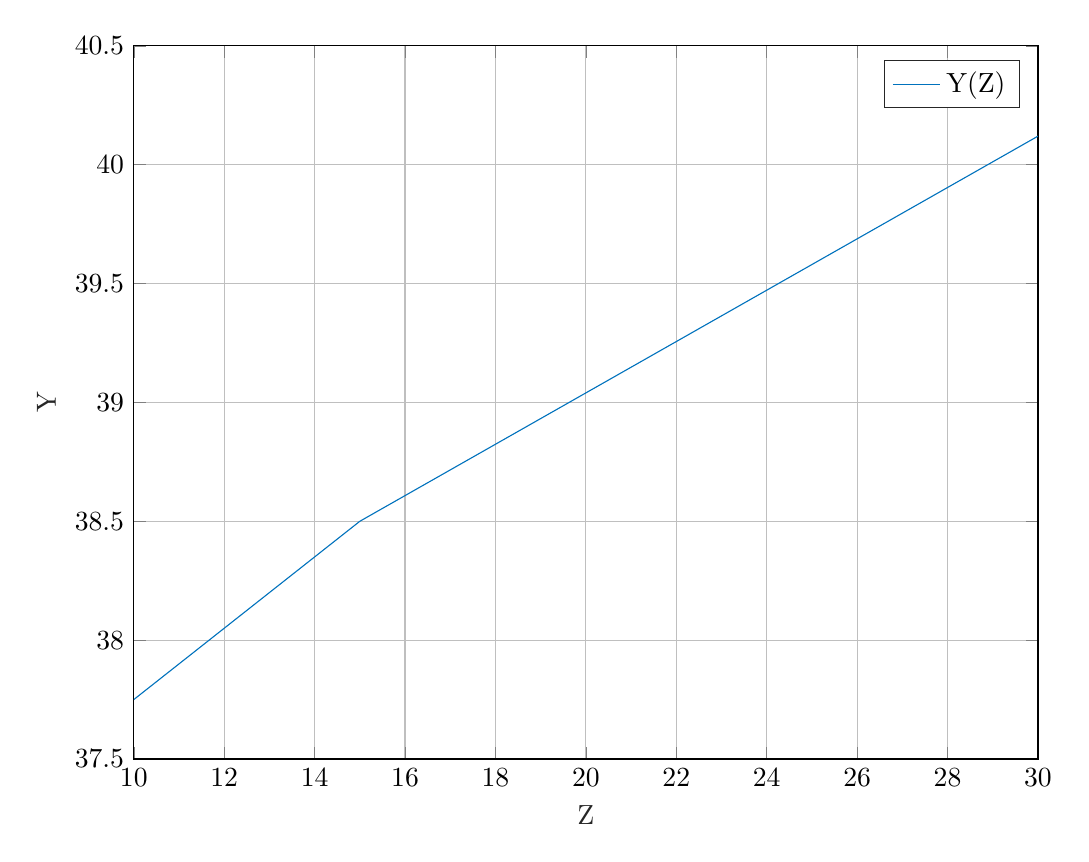
\begin{tikzpicture}

\begin{axis}[%
width=4.521in,
height=3.566in,
at={(0.758in,0.481in)},
scale only axis,
xmin=10,
xmax=30,
xlabel style={font=\color{white!15!black}},
xlabel={Z},
ymin=37.5,
ymax=40.5,
ylabel style={font=\color{white!15!black}},
ylabel={Y},
axis background/.style={fill=white},
xmajorgrids,
ymajorgrids,
legend style={legend cell align=left, align=left, draw=white!15!black}
]
\addplot [color=mycolor1]
  table[row sep=crcr]{%
10	37.75\\
15	38.5\\
30	40.12\\
};
\addlegendentry{Y(Z)}

\end{axis}
\end{tikzpicture}%
    \caption{Charakterystyka statyczna obiektu}
    \label{lab:zad2:zad2charStat:figure}
 \end{figure}

 Charakterystyka statyczna pokazuje, że właściwości statyczne obiektu nie są
liniowe, wartości sygnału wyjściowego w zależności od sygnały wejściowego nie
zachowują się liniowo.

\newpage
